\chapter{Experiment}
\section{Path}
The path system has successfully been tested in the field 
\subsection{Landing path with pixhawk autopilot}
A landing path was create with the goal of testing the concept of the landing path system. The test was perform with the pixhawk autopilot, and navigation system. Thus high performance from the X8 is not expected. The path was create in cooperation with the operator and pilot, which dictated the maximum size of the landing path.

The height where the \gls{uav} held after the approach path was to low, and during a real landing would cause the \gls{uav} to crash. Thus either the length of the landing path or the glide slope angle has to increase. The performance of the pixhawk autopilot was not adequate to successfully hit the net.

The wind condition was measured to be $5m/s$ from the north, which caused the \gls{uav} to have to perform the landing with a cross wind.

The path was created with manually deciding the rotation directions, due to the start position and where the operator wanted the \gls{uav} to circle down to the correct height. In this case the shortest path would bring the \gls{uav} close to a no-fly zone


\begin{figure}[H]
	\centering
		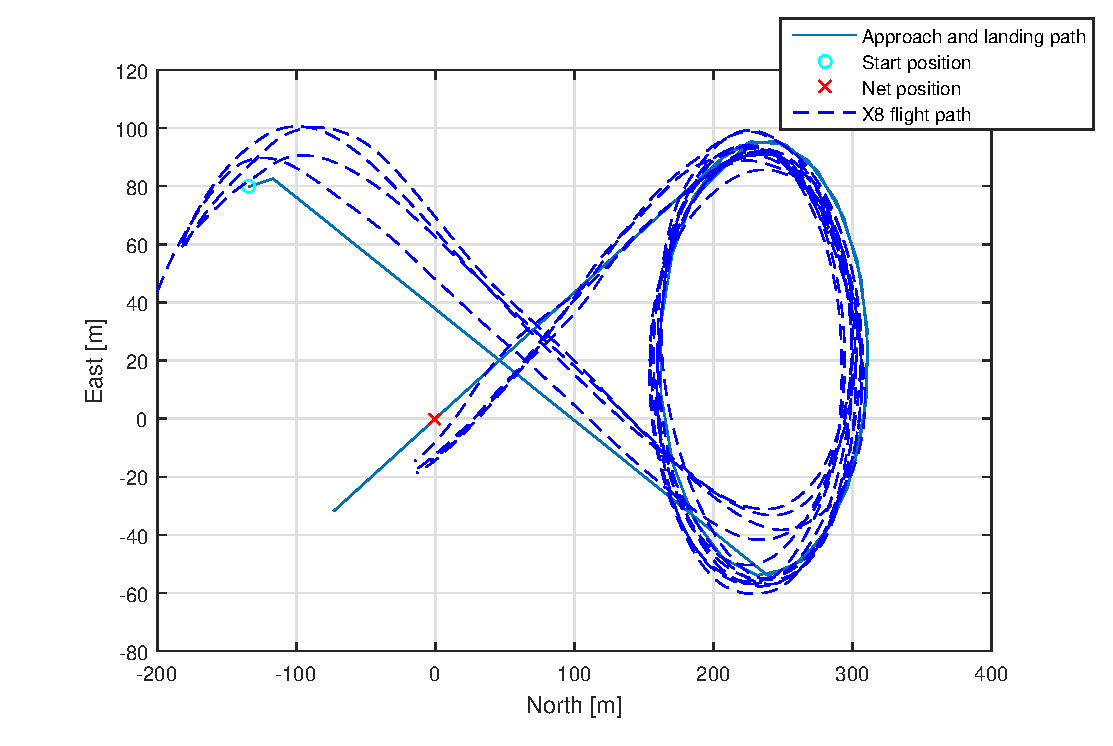
\includegraphics[width=1\textwidth]{figs/Experiment/NorthEastLandingPathArdu.eps}
		\caption{Four lateral flight paths towards the net position}
		\label{Fig:NorthEastArdu}
\end{figure}
\subsection*{Landing path with DUNE control system}
The autonomous landing system was tested with DUNE controllers in the field on two separated days.

Wind condition $8 m/s$
\section{Navigation}
The navigation system was tested in both a X8 and in a multicopter system.

\subsection{Formation position}
The accuracy of the \gls{rtk-gps} position system was tested with two mutlicopter system, with the goal of measuring the distance between them. During stationary conditions it was determined that \gls{rtk-gps} was highly accurate, and is required when performing a formation flight. The same principle is used in determining the net position, where the net nest apply \gls{rtk-gps} to determine it's own position. However currently the position has to manually be written to Neptus, which must change when performing a ship landing.
\subsection{Short loss compensator}
Include result when short loss was not in use. Compare to result when it's in use.

The short loss compensator bring the position solution from the pixhawk close enough to the \gls{rtk-gps} solution such that the navigation system does not lose its position. However a highly aggressive control system that attempt to keep the error at centimeter level is expected to react to the discontinues introduced from the compensator. All though currently it has not been concluded that the compensator cause problems for the control system, since failure has happen during demanding wind condition. 